%%%%%%%%%%%%%%%%%%%%%%%%%%%%%%%%%%%%%%%%%%%%%%%%%%%%%%%%%%%%%%%
\documentclass[11pt]{article}

\usepackage[utf8]{inputenc}
\usepackage[margin=1in]{geometry} 
\usepackage{amsmath,amsfonts,amsthm,amssymb,bm}

\usepackage{graphicx}
\usepackage{listings}
\usepackage[dvipsnames]{xcolor}
\usepackage{subcaption}
\usepackage{mdframed}
\usepackage{multicol}
\usepackage{environ}
\usepackage{tikz, pgfplots}
\usepackage{framed}

\newenvironment{EX}[2][Exercise]{\begin{trivlist}
\item[{\color{red} \hskip \labelsep {\bfseries #1}\hskip \labelsep {\bfseries #2.}}]}{\end{trivlist}}

\newenvironment{SL}[1][Solution]{\begin{trivlist}
\item[{\color{blue} \hskip \labelsep {\bfseries #1:}}]}{\end{trivlist}}

\lstdefinestyle{mystyle}{
    backgroundcolor=\color{Gray!25!white},
    commentstyle=\color{PineGreen},
    keywordstyle=\color{Red},
    basicstyle=\footnotesize\ttfamily,
    breakatwhitespace=false,
    showstringspaces=false,
    showspaces=false,
    showtabs=false,
    breaklines=true,
    keepspaces=true,
    captionpos=b,
    numbers=left,
    numbersep=5pt,
    tabsize=2
}
\lstset{style=mystyle}

\graphicspath{ {figs/} }

\usepackage{fourier} 
\usepackage{array}
\usepackage{makecell}

\renewcommand\theadalign{bc}
\renewcommand\theadfont{\bfseries}
\renewcommand\theadgape{\Gape[4pt]}
\renewcommand\cellgape{\Gape[4pt]}

\begin{document}

% --------------------------------------------------------------
% Start here
% --------------------------------------------------------------
\setcounter{secnumdepth}{1}
\setcounter{tocdepth}{1}

\noindent {\Large \textbf{Aluno:} Otacílio Bezerra L. N. (385213)} \hfill {\Large \bfseries TI0119: AP2 - Resumo (Extra)} 

\noindent\rule{4cm}{0.4pt} \vskip0.5cm

{\center{\Large \bf Estruturas para Sistemas de Tempo Discreto} \\}

\section{Introdução}

Nesse documento encontra-se um resumo para o arquivo \texttt{``estruturas\_sistemas\_discreto.pdf''}. O arquivo em questão discute representações gráficas e estruturas básicas para representar sistemas lineares e invariantes no tempo (sistemas LIT), especificamente para o caso discreto. O objetivo dessas representações consiste tanto em proporcionar uma forma sistemática de descrever a analisar os sistemas, como também permitir maior facilidade na implementação desses sistemas utilizando componentes de \textit{hardware}. Esses sistemas são comumente definidos através de funções de transferência, $H(z)$, ou de uma equivalente equação de diferenças, comumente para $y[n]$, nas formas gerais:
\begin{equation} \label{eq:sistemas}
\begin{matrix}
	H(z) = \cfrac{\displaystyle\sum_{j = 0}^{M} \beta_j z^{-j}}{\displaystyle\sum_{k = 0}^{N} \alpha_k z^{-k}}
	& & \text{e} & &
	y[n] = \displaystyle\sum_{k=1}^{N} \alpha_k y[n-k] + \displaystyle\sum_{k=0}^{M} \beta_k x[n-k].
\end{matrix}
\end{equation} 

\noindent Notamos na equação anterior que a implementação dessas equações exigem três operações básicas: \textit{adição de sequências}, \textit{multiplicação de uma sequência por uma constante} e \textit{atraso}. Essas operações são representadas graficamente na Figura \ref{fig:operations}.

\begin{figure}[ht] \centering
	\begin{subfigure}[b]{0.3\textwidth}
		\resizebox{\textwidth}{!}{\tikzset{every picture/.style={line width=0.75pt}} %set default line width to 0.75pt        

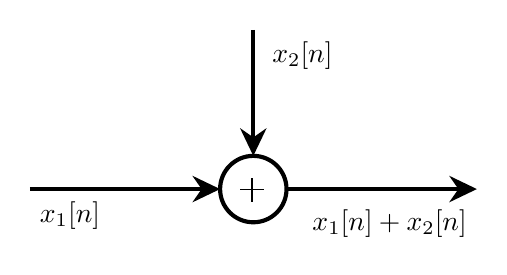
\begin{tikzpicture}[x=0.75pt,y=0.75pt,yscale=-1,xscale=1]
%uncomment if require: \path (0,229.28334045410156); %set diagram left start at 0, and has height of 229.28334045410156

%Shape: Circle [id:dp36745056819088584] 
\draw  [line width=1.5]  (120.33,107.33) .. controls (120.33,98.5) and (127.5,91.33) .. (136.33,91.33) .. controls (145.17,91.33) and (152.33,98.5) .. (152.33,107.33) .. controls (152.33,116.17) and (145.17,123.33) .. (136.33,123.33) .. controls (127.5,123.33) and (120.33,116.17) .. (120.33,107.33) -- cycle ;
\draw   (130,107.69) -- (141.38,107.69)(135.69,102) -- (135.69,113.38) ;
%Straight Lines [id:da7922750538103807] 
\draw [line width=1.5]    (152.33,107.33) -- (241.05,107.33) ;
\draw [shift={(244.05,107.33)}, rotate = 180] [fill={rgb, 255:red, 0; green, 0; blue, 0 }  ][line width=1.5]  [draw opacity=0] (13.4,-6.43) -- (0,0) -- (13.4,6.44) -- (8.9,0) -- cycle    ;

%Straight Lines [id:da25310615160739736] 
\draw [line width=1.5]    (136.33,30.57) -- (136.33,88.33) ;
\draw [shift={(136.33,91.33)}, rotate = 270] [fill={rgb, 255:red, 0; green, 0; blue, 0 }  ][line width=1.5]  [draw opacity=0] (13.4,-6.43) -- (0,0) -- (13.4,6.44) -- (8.9,0) -- cycle    ;

%Straight Lines [id:da210821574381732] 
\draw [line width=1.5]    (28.62,107.33) -- (117.33,107.33) ;
\draw [shift={(120.33,107.33)}, rotate = 180] [fill={rgb, 255:red, 0; green, 0; blue, 0 }  ][line width=1.5]  [draw opacity=0] (13.4,-6.43) -- (0,0) -- (13.4,6.44) -- (8.9,0) -- cycle    ;


% Text Node
\draw (48,120) node   {$x_{1}[ n]$};
% Text Node
\draw (202,124) node   {$x_{1}[ n] +x_{2}[ n]$};
% Text Node
\draw (160,43) node   {$x_{2}[ n]$};


\end{tikzpicture}
}
		\caption{}
	\end{subfigure}%
	\hfill
	\begin{subfigure}[b]{0.3\textwidth}
		\resizebox{\textwidth}{!}{\tikzset{every picture/.style={line width=0.75pt}} %set default line width to 0.75pt        

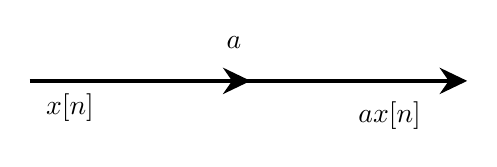
\begin{tikzpicture}[x=0.75pt,y=0.75pt,yscale=-1,xscale=1]
%uncomment if require: \path (0,229.28334045410156); %set diagram left start at 0, and has height of 229.28334045410156

%Straight Lines [id:da210821574381732] 
\draw [line width=1.5]    (21.62,98.33) -- (125,98.33) ;
\draw [shift={(128,98.33)}, rotate = 180] [fill={rgb, 255:red, 0; green, 0; blue, 0 }  ][line width=1.5]  [draw opacity=0] (13.4,-6.43) -- (0,0) -- (13.4,6.44) -- (8.9,0) -- cycle    ;

%Straight Lines [id:da820799252153864] 
\draw [line width=1.5]    (126,98.33) -- (229.38,98.33) ;
\draw [shift={(232.38,98.33)}, rotate = 180] [fill={rgb, 255:red, 0; green, 0; blue, 0 }  ][line width=1.5]  [draw opacity=0] (13.4,-6.43) -- (0,0) -- (13.4,6.44) -- (8.9,0) -- cycle    ;


% Text Node
\draw (41,111) node   {$x[n]$};
% Text Node
\draw (195,115) node   {$ax[n]$};
% Text Node
\draw (120,80) node   {$a$};


\end{tikzpicture}
}
		\caption{}
	\end{subfigure}%
	\hfill
	\begin{subfigure}[b]{0.3\textwidth}
		\resizebox{\textwidth}{!}{

\tikzset{every picture/.style={line width=0.75pt}} %set default line width to 0.75pt        

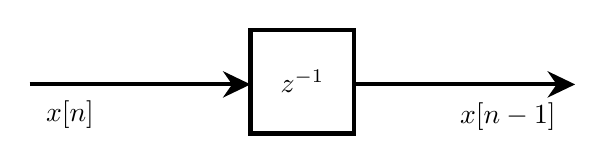
\begin{tikzpicture}[x=0.75pt,y=0.75pt,yscale=-1,xscale=1]
%uncomment if require: \path (0,229.28334045410156); %set diagram left start at 0, and has height of 229.28334045410156

%Straight Lines [id:da210821574381732] 
\draw [line width=1.5]    (36.62,90.33) -- (140,90.33) ;
\draw [shift={(143,90.33)}, rotate = 180] [fill={rgb, 255:red, 0; green, 0; blue, 0 }  ][line width=1.5]  [draw opacity=0] (13.4,-6.43) -- (0,0) -- (13.4,6.44) -- (8.9,0) -- cycle    ;

%Straight Lines [id:da820799252153864] 
\draw [line width=1.5]    (193,90.33) -- (296.38,90.33) ;
\draw [shift={(299.38,90.33)}, rotate = 180] [fill={rgb, 255:red, 0; green, 0; blue, 0 }  ][line width=1.5]  [draw opacity=0] (13.4,-6.43) -- (0,0) -- (13.4,6.44) -- (8.9,0) -- cycle    ;

%Shape: Square [id:dp7779976189799176] 
\draw  [line width=1.5]  (143,64) -- (193,64) -- (193,114) -- (143,114) -- cycle ;

% Text Node
\draw (56,105) node   {$x[ n]$};
% Text Node
\draw (267,106) node   {$x[ n-1]$};
% Text Node
\draw (168,89) node   {$z^{-1}$};


\end{tikzpicture}
}
		\vskip0.15cm
		\caption{}
	\end{subfigure}

	\caption{Representação gráfica das operações entre sinais discretos.}
	\label{fig:operations}
\end{figure}

\section{Representação em Diagrama de Blocos} 

Considere um sistema descrito por uma equação de diferenças genérica como a exposta em \eqref{eq:sistemas}. Podemos representar o sistema através de um diagrama de blocos genérico tal qual representado na Figura \ref{fig:direta1}. Esse diagrama é uma realização direta da equação de diferenças, sendo cada cadeia de blocos representativo de um somatório da fórmula.

[img]

Esse formato, denominado de \textit{Forma Direta I}, define uma variável $v[n]$ que equivale a
\begin{equation}
	v[n] = \sum_{k=0}^{M} \beta_k x[n-k].
\end{equation}

\noindent No domínio $\mathbb{Z}$, teremos a seguinte representação para a transformada dos sinais $v[n]$ e $y[n]$:
\begin{equation}
\begin{matrix}
	V(z) = \underbrace{\left( \displaystyle\sum_{k=0}^M \beta_k z^{-k} \right)}_{H_1(z)} X(z); & & Y(z) = \underbrace{\cfrac{1}{1 - \left( \displaystyle\sum_{k=1}^M \alpha_k z^{-k} \right)} }_{H_2(z)} V(z)
\end{matrix},
\end{equation}

\noindent o que implica que $Y(z) = H_2(z) \left[ H_1(z) X(z) \right] = H_1(z) \left[ H_2(z) X(z) \right]$. Considerando $W(z) = H_2(z) X(z)$, podemos obter a mesma equação de diferenças anterior agora na forma:
\begin{equation}
\begin{matrix}
	w[n] = \displaystyle\sum_{k=1}^N \alpha_k w[n-k] + x[n]; & & y[n] = \displaystyle\sum_{k=0}^M \beta_k w[n-k]
\end{matrix}.
\end{equation} 

\noindent Essa forma alternativa para as equações sugere uma topologia para o diagrama de blocos no formato da Figura \ref{fig:direta2}. Essa fórmula é denominada de \textit{Forma Direta II}.

[img]

As duas formas anteriormente derivada são semelhantes, com exceção de uma inversão entre as constantes de multiplicação. No entanto, nota-se que os mesmos sinais $w[n-k]$ são representados de forma repetida na cadeia esquerda e direita do diagrama de blocos. Isso evidencia a possibilidade de uma simplificação dessa representação para um diagrama de blocos de cadeia única, que reduz a complexidade de implementação desse sistema. Essa nova forma, apresentada na Figura \ref{fig:diretaCanonica}, é denominada de \textit{Forma Direta II Canônica}.

[img]

\section{Representação em Diagrama de Fluxo de Sinais}

Uma outra representação gráfica para sistemas LIT consiste nos diagramas (ou grafos) de fluxo. Essa representação consiste num conjunto de nós e ramos interconectados, no qual cada nó representa um sinal e um ramo, possivelmente associado a um peso, indica a direção do fluxo desse sinal (ou o valor de sinais que entram nesse nó). Nesses diagramas, os ramos que incidem sobre um nó são somados para compor o valor do sinal naquele ponto, e esse valor é transmitido pelos ramos que incidem a partir desse nó. A Figura \ref{fig:flux01} demonstra um caso genérico de um diagrama de fluxo mostrando um nó de origem (sobre o qual não incide nenhum ramo), um nó de saída (que não possui nenhum ramo de sáida) e os nós intermediários.

[img]

Uma vez que o Diagrama de Fluxo representa a mesma informação que um Diagrama de Bloco, é sempre possível obter uma representação equivalente entre essas duas formas ao substituir um bloco de soma por um nó, e um bloco de atraso por um ramo carregando a variável $z^{-1}$. Dessa forma, é sempre possível obter \textit{Formas Direta I} e \textit{Formas Diretas II} utilizando essa notação, como demonstrado na Figura \ref{fig:flux02}.

[img]

\section{Estruturas Básicas para Sistemas IIR}

Além da \textit{Forma Direta I} e da \textit{Forma Direta II}, existem também outras possibilidades de representar um Sistema IIR. 

\subsection{Formas em Cascata}

Considere a função de transferência genérica exposta em \eqref{eq:sistemas}. Considere, agora, a seguinte fatoração:
\begin{equation}
	H(z) = A \cfrac{\displaystyle\prod_{k=1}^{M_1}\left( 1 - f_k z^{-1} \right) \displaystyle\prod_{k=1}^{M_2}\left( 1 - g_k z^{-1} \right) \left( 1 - g^*_k z^{-1} \right)}{\displaystyle\prod_{k=1}^{N_1}\left( 1 - c_k z^{-1} \right) \displaystyle\prod_{k=1}^{N_2}\left( 1 - d_k z^{-1} \right) \left( 1 - d^*_k z^{-1} \right)},
\end{equation}

\noindent onde $M = M_1 + 2*M_2$ e $N = N_1 + 2*N_2$. Nessa representação, os fatores $f_k$ e $c_k$ estão associados com os polos e zeros reais do sistema, enquanto $(g_k, g^*_k)$ e $(d_k, d^*_k)$ são os fatores associados aos pares de zeros e polos complexos conjugados. Essa formulação sugere a possibilidade de representar o sistema com um estrutura modular em cascata de sistemas de primeira e segunda ordem. Um formato específico em cascata, por exemplo, consiste na implementação baseada em secções de segunda ordem, obtido ao combinar pares de fatores reais e/ou pares de complexos conjugados:
\begin{equation}
\begin{matrix}
	H(z) = \displaystyle\prod_{k=1}^{N_s} \cfrac{\beta_0 + \beta_{1k} z^{-1} + \beta_{2k} z^{-2}}{1 - \alpha_{1k} z^{-1} - \alpha_{2k} z^{-2}},
\end{matrix}
\end{equation}

\noindent onde $N_s = \left\lfloor (N+1) / 2 \right\rfloor$ e assumimos que o sistema é causal ($M \leq N$). Para construir uma representação gráfica, podemos considerar a \textit{Forma Direta II Canônica} e as equações de diferenças associadas à função de transferência anterior. O diagrama, apresentado na Figura \ref{fig:cascata} para o caso de $N = 6$, é resultado da aplicação às equações
\begin{align}
	y_0[n] &= x[n], \\
	w_k[n] &= \alpha_{1k} w_k[n-1] + \alpha_{2k} w_k[n-2] + y_{k-1}[n],\ k = 1, 2, \cdots, N_s, \\
	y_k[n] &= \beta_{0k} w_k[n] + \beta_{1k} w_k[n-1] + \beta_{2k} w_{k}[n-2],\ k = 1, 2, \cdots, N_s, \\
	y[n] &= y_{N_s}[n].
\end{align}

[img]

\subsection{Forma Paralela}

Uma função de transferência racional com coeficientes reais pode ser expressa da seguinte forma:
\begin{equation}
	H(z) = \sum_{k=0}^{N_p} C_k z^{-k} + \sum_{k=1}^{N_1} \cfrac{A_k}{1 - c_k z^{-1}} + \sum_{k=1}^{N_2} \cfrac{B_k(1 - e_k z^{-1})}{(1 - d_k z^{-1})(1 - d^*_k z^{-1})} = \sum_{k=0}^{N_p} C_k z^{-k} + \sum_{k=1}^{N_s} \cfrac{(e_{0k} + e_{1k} z^{-1})}{(1 - \alpha_{1k} z^{-1} - \alpha_{2k} z^{-2})}
\end{equation}

\noindent onde $N = N_1 + 2N_2$, $N_p = M - N$ e $N_s = \left\lfloor (N+1) / 2 \right\rfloor$. Essa representação implica numa outra forma alternativa, denominada de \textit{Forma Paralela}, para a representação de sistemas, indicada pela soma de $N_p$ secções de multiplicação simples em paralelo com $N_s$ secções de segunda-ordem com um zero. A Figura \ref{fig:paralelo} exemplifica o diagrama para o caso $M = N = 6$.

[img]

\subsection{Formas Transpostas}

Um procedimento comum utilizado para transformar diagramas de fluxo em formas equivalentes é o denominado de \textit{Transposição} ou \textit{Diagramas de Fluxo Reverso}. A \textit{Transposição} pode ser aplicado a qualquer uma das estruturas discutidas anteriormente, e tem o efeito de inverter a ordem sobre a qual os componentes são implementados. O procedimento é descrito pelos passos:

\begin{enumerate}
	\item Inverta as direções de todos os ramos da rede;
	
	\item Mantenha as transmitâncias (ganhos) dos ramos;
	
	\item Troque os papéis da entrada e da saída (nós fontes se tornam nós de saída e vice-versa).
\end{enumerate}

A Figura \ref{fig:transposta} exemplifica o efeito da \textit{Transposição} para um sistema de primeira ordem e um sistema de segunda ordem, respectivamente.

[img]

\section{Estruturas Básicas para Sistemas FIR}

As estruturas de um Sistema de Resposta ao Impulso Finito (Sistema FIR) podem ser consideradas como caso particulares das estruturas para os sistemas IIR. No caso de um Sistema FIR, a função de transferência possui apenas zeros (exceto os polos em $z = 0$), e possui a forma:
\begin{equation}
	y[n] = \sum_{k=0}^M \beta_k x[n-k].
\end{equation} 

\subsection{Forma Direta}

A representação gráfica da Forma Direta pode ser obtida simplesmente ao excluir as cadeias relacionadas aos fatores dos polos da representação apresentada anteriormente. Um exemplo dessa aplicação é mostrada na Figura \ref{fig:diretaFIR}.

[img]

\subsection{Forma em Cascata}

Para obter uma forma em cascata, a função de transferência de um Sistema FIR pode ser fatorada da seguinte forma:
\begin{equation}
	H(z) = \sum_{n=0}^{M} = \prod_{k=1}^{M_s}\left( \beta_{0k} + \beta{1k} z^{-1} + \beta{2k} z^{-2} \right),
\end{equation}

\noindent em que $M_s = \left\lfloor (M+1) / 2 \right\rfloor$. Um exemplo do diagrama de fluxo em cascata é disposto na Figura \ref{fig:cascataFIR}.

[img]

\subsection{Sistemas FIR com Fase Generalizada} 

Dentre os sistemas LTI que apresentam fase linear generalizada, destacam-se os sistemas FIR do tipo:
\begin{equation}
	h[n] = \pm h[M - n],\ n = 0, 1, \cdots, M.
\end{equation}

Existem quatro possíveis categorias para sistemas dessa forma: Tipo I, Tipo II, Tipo III e Tipo IV. As categorias I e II são definidas para $h[M-n]$ positivo, mas com $M$ par e ímpar respectivamente. Já as categorias II e IV são definidas para $h[M-n]$ negativo, com $M$ par e ímpar respectivamente. Aplicando a fórmula de sistema FIR com fase linear generalizada à forma genérica da equação de diferenças resulta nas fórmulas:
\begin{align}
y[n] = \begin{cases}
	 \displaystyle\sum_{k=0}^{M/2-1} h[k](x[n-k]+x[n-M+k])+h[M/2]x[n-M/2] & \text{(Tipo I)} \\
	 \displaystyle\sum_{k=0}^{(M-1)/2} h[k](x[n-k]+x[n-M+k]) & \text{(Tipo II)} \\
	 \displaystyle\sum_{k=0}^{M/2-1} h[k](x[n-k]-x[n-M+k])+h[M/2]x[n-M/2] & \text{(Tipo III)} \\
	 \displaystyle\sum_{k=0}^{(M-1)/2} h[k](x[n-k]-x[n-M+k]) & \text{(Tipo IV)}
\end{cases}
\end{align}

Os diagramas equivalentes para as equações acima são apresentadas na Figura \ref{fig:faseGeneralizada}.

[img]

% --------------------------------------------------------------
% Stop here
% --------------------------------------------------------------

\end{document}